\documentclass[landscape]{article}
\usepackage[a4paper,margin=1cm]{geometry}
\usepackage[utf8]{inputenc}
\usepackage[T1]{fontenc}
\usepackage{multicol}
\usepackage{xcolor,colortbl}
\usepackage{lipsum}
\usepackage{amsmath}
\usepackage{enumitem}
\usepackage{forest}
\forestset{qtree/.style={for tree={parent anchor=south, 
           child anchor=north,align=center}}}

\usepackage{graphicx}
\graphicspath{ {./images/} }

\setlength{\columnsep}{1cm}
\renewcommand{\columnseprulecolor}{\normalcolor}
% set \paragraph vertical spacing
\makeatletter
\renewcommand{\paragraph}{\@startsection{paragraph}{4}{\z@}%
                                    {1.5ex}%
                                    {-0.75em}%
                                    {\normalfont\normalsize\bfseries}}
\makeatother
% reduce space before \subparagraph
\makeatletter
\renewcommand{\subparagraph}{\@startsection{subparagraph}{5}{\z@}%
                                       {1ex}%
                                       {-0.75em}%
                                       {\normalfont\normalsize\bfseries\hspace{1.25em}}}% Add \hspace{1.25em} for 1 level of indent
\makeatother
% add vertical space before \minipage and rename environment to \minipage
\let\oldminipage\minipage
\let\endoldminipage\endminipage
\renewenvironment{minipage}{\vspace{0.5em}\begin{oldminipage}{0.925\linewidth}}{\end{oldminipage}}

% Custom command for horizontal separator
\newcommand{\sep}{\noindent\rule{\linewidth}{0.5pt}}

\pagenumbering{gobble}

\begin{document}
\begin{multicols*}{3}
    \footnotesize

    \section*{ARO - Architecture des Ordinateurs \\ \small{Leonard Cseres - Avril 2024}}
    \begin{tabular*}{\linewidth}{@{\extracolsep{\fill}} ccc}
        \hline
        \textbf{Hex} & \textbf{Bytes (B)}                            & \textbf{Bits (b)} \\
        \hline
        0x400        & $1\text{KB} = 2^{10}\text{B} = 1024\text{B}$  & 8Kb               \\
        0x800        & $1\text{MB} = 2^{20}\text{B} = 1024\text{KB}$ & 8Mb               \\
        0x1000       & $1\text{GB} = 2^{30}\text{B} = 1024\text{MB}$ & 8Gb               \\
        0x2000       & $1\text{TB} = 2^{40}\text{B} = 1024\text{GB}$ & 8Tb               \\
        \hline
    \end{tabular*}\\\\\\
    \begin{minipage}
        \centering
        \textbf{Conversion hexadécimal $\rightarrow$ binaire}\\\vspace{0.5em}
        \begin{tabular}[h]{cc|cc|cc}
            0x0 & 0000 & 0x6 & 0110 & 0xC & 1100 \\
            0x1 & 0001 & 0x7 & 0111 & 0xD & 1101 \\
            0x2 & 0010 & 0x8 & 1000 & 0xE & 1110 \\
            0x3 & 0011 & 0x9 & 1001 & 0xF & 1111 \\
            0x4 & 0100 & 0xA & 1010 &     &      \\
            0x5 & 0101 & 0xB & 1011 &     &      \\
        \end{tabular}
    \end{minipage}

    \begin{forest}
        for tree={edge={->}}
        [\textbf{Non-Signé}
        [\texttt{ADD} $> 2^n-1$
            [C (\textit{carry})]
        ]
        [\texttt{SUB} $< 0$
            [B (\textit{borrow})]
        ]
        ]
    \end{forest}
    \begin{forest}
        for tree={edge={->}}
        [\textbf{Signé}
        [$< -2^{n-1}$ ou $> 2^{n-1}-1$
        [V (\textit{overflow})]
        ]
        ]
    \end{forest}

    \begin{forest}
        for tree={edge={->}, qtree}
        [\textbf{CPU}\\(Contrôle/traite/execute)
        [Mémoire $\Longleftrightarrow$ Unité de \textbf{contrôle}]
            [Unité de \textbf{traitement}\\(ALU/Registres)]
        ]
    \end{forest}

    \begin{forest}
        for tree={edge={->}, qtree}
        [\textbf{Mémoire}
        [volatile\\(RAM/SRAM)]
        [non-volatile\\(flash memory)]
        ]
    \end{forest}

    \sep

    \paragraph{Von Neumann} Architecture avec un seul bus pour les données et les instructions

    \paragraph{Harvard} Architecture avec deux bus séparés pour les données et les instructions

    \paragraph{Adressage} $A_{fin} = A_{debut} + T - 1$ où $T$ est la taille de la zone d'adressage

    \paragraph{Endianness} \textit{Big Endian} (octet de poids fort en premier), \textit{Little Endian} (octet de poids faible en premier)

    \paragraph{Alignement (Mem. 64-bits)}\mbox{}\\
    \begin{tabular}[h]{|c|>{\columncolor{blue!40}}c|c|>{\columncolor{red!40}}c|c|>{\columncolor{green!40}}c|c|>{\columncolor{red!40}}c|c|}
        \hline
                          & \textbf{0} & \textbf{1} & \textbf{2} & \textbf{3} & \textbf{4} & \textbf{5} & \textbf{6} & \textbf{7} \\
        \hline
        \textbf{00000000} & 00         & 00         & 00         & 00         & 00         & 00         & 00         & 00         \\
        \textbf{00000008} & 00         & 00         & 00         & 00         & 00         & 00         & 00         & 00         \\
        \textbf{00000010} & 00         & 00         & 00         & 00         & 00         & 00         & 00         & 00         \\
        \textbf{\dots}    & \dots      & \dots      & \dots      & \dots      & \dots      & \dots      & \dots      & \dots      \\
        \hline
    \end{tabular}\\\\
    \begin{tabular}[h]{llllll}
        \cellcolor{blue!40} & 64 bits word & \cellcolor{green!40} & 32 bits word & \cellcolor{red!40} & 16 bits word \\
    \end{tabular}

    % TODO: Memory PROM

    \paragraph{Types d'Instructions}
    \begin{itemize}
        \item Instruction de \textbf{calcul/traitement}
        \item Instruction de \textbf{transfert de données}
        \item Instruction de \textbf{contrôle} (branchement, saut, interruption)
    \end{itemize}

    \sep

    \paragraph{Registres} accès rapide (plus que la mémoire), stockage temporaire, passage de paramètres, sauvegarde de contexte\mbox{}\vspace{0.5em}\\
    \begin{minipage}
        \centering
        \begin{tabular}[h]{|c|c|}
            \hline
            \textbf{Registres} & \textbf{Fonction}                             \\
            \hline
            \texttt{SP}        & Pointeur de pile                              \\
            \texttt{LR}        & Registre de lien (appel de fct, interruption) \\
            \texttt{PC}        & Compteur de programme                         \\
            \texttt{CPSR}      & Registre d'état                               \\
            \hline
        \end{tabular}
    \end{minipage}

    \begin{minipage}
        \centering
        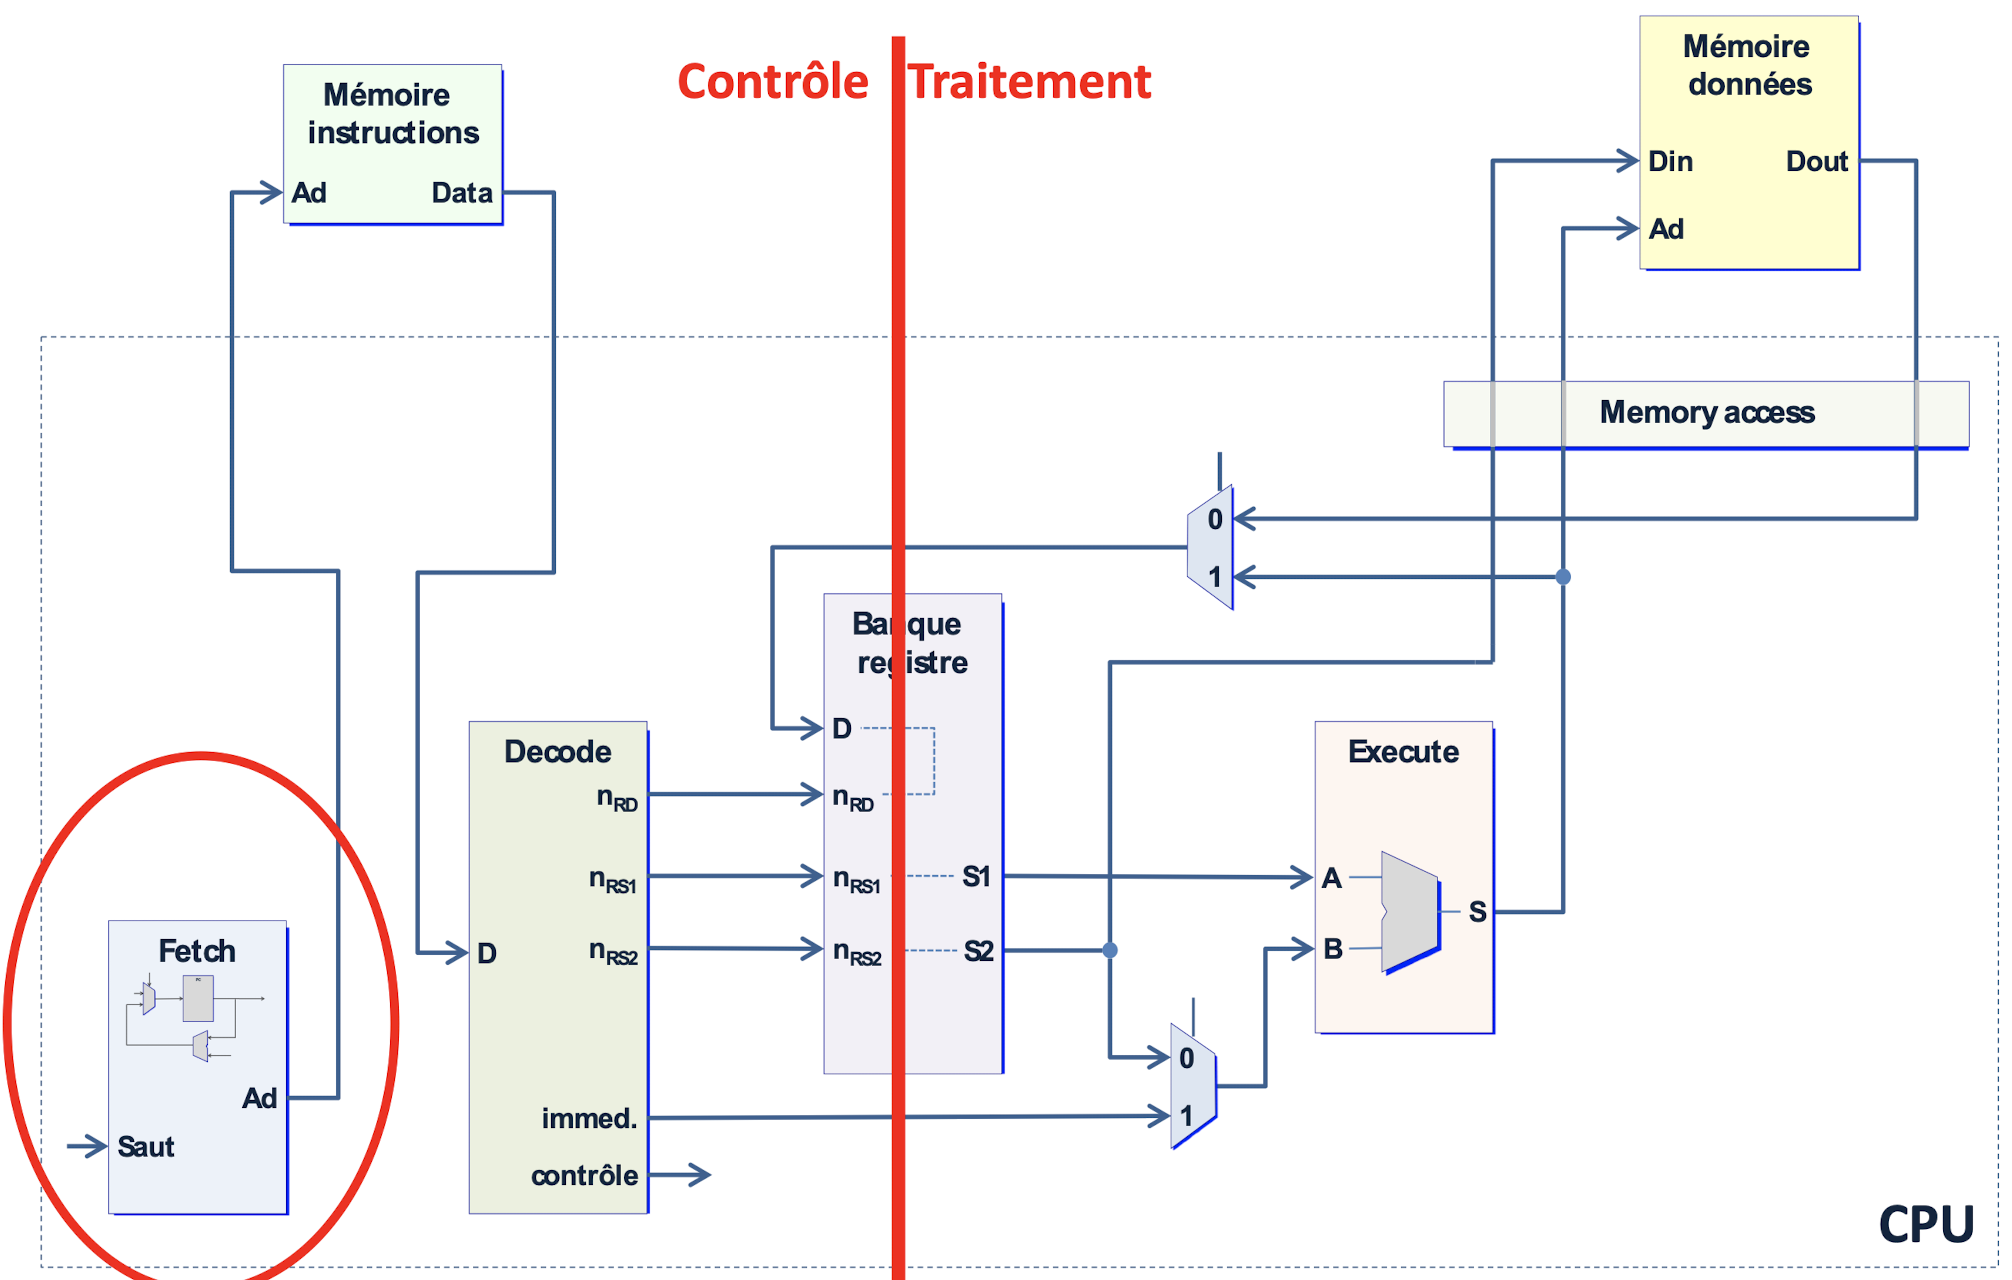
\includegraphics[width=\linewidth]{arch.png}
    \end{minipage}

    \paragraph{Fetch} Récupération de l'instruction à exécuter

    \subparagraph{PC} Correspond au nombre de bytes de l'instruction, \textit{indépendamment du bus d'adresses}\mbox{}\vspace{0.5em}\\
    \begin{minipage}
        \hspace{1em}
        \begin{tabular*}{\linewidth}{@{\extracolsep{\fill}}|c|ccc|}
            \hline
            \textbf{Bits d'instruction} & 8 bits & 16 bits & 32 bits \\
            \hline
            \textbf{Incrément}   & 1      & 2       & 4       \\
            \hline
        \end{tabular*}
    \end{minipage}


    \subparagraph{Sauts} $A_{\textit{fut}} = A_{PC} + \texttt{extension\_16bits}(\textit{offset}_{11} \cdot 2) + 4$  avec $\textit{offset}_{11}$ signé et \texttt{extension\_16bits} garde le signe

    \subparagraph{Vecteur d'interruption} $A_{\textit{vec}} = A_{\textit{base}} + (C \cdot N)$ avec $C$ le numéro de l'interruption et $N$ le nbr. de bytes du bus d'instructions

    \begin{minipage}
        \centering
        \begin{tabular}[h]{|c|c|}
            \hline
            \textbf{ISR} & \textbf{Adresse Vecteur}          \\
            \hline
            0x00000      & $A_{\textit{base}}$               \\
            \dots        & $A_{\textit{base}} + (1 \cdot N)$ \\
            \hline
        \end{tabular}
    \end{minipage}

    \paragraph{Decode} Décodage de l'instruction pour déterminer l'opération à effectuer
    % TODO: \subparagraph{Banque de registres}
    \subparagraph{CSPR}
    \begin{itemize}
        \item \texttt{N} (Negative) : résultat négatif
        \item \texttt{Z} (Zero) : résultat nul
        \item \texttt{C} (Carry) : retenue
        \item \texttt{V} (Overflow) : dépassement
        \item \texttt{IF} (Interrupt Flag) : autorisation d'interruption
        \item \texttt{T} (Thumb) : jeu d'instructions
        \item \texttt{M} (Mode) : mode d'exécution
    \end{itemize}

    \sep

    \paragraph{Utilisation de la pile} \texttt{PUSH} et \texttt{POP}
    \begin{itemize}
        \item Stockage des adresses de retour
        \item Sauvegarde des registres
        \item Stockage des variables locales
    \end{itemize}

    \paragraph{ARM Thumb}\mbox{}\vspace{0.5em}\\
    \begin{minipage}
        \centering
        \begin{tabular}[h]{|c|c|}
            \hline
            \textbf{Mnemonic} & \textbf{Instruction}   \\
            \hline
            \texttt{ADC}      & Add with carry         \\
            \texttt{B}        & Unconditional branch   \\
            \texttt{Bxx}      & Conditional branch     \\
            \texttt{BL}       & Branch with link       \\
            \texttt{BX}       & Branch and exchange    \\
            \texttt{CMN}      & Compare negative       \\
            \texttt{LDR}      & Load word              \\
            \texttt{LDRB}     & Load byte              \\
            \texttt{LDRH}     & Load halfword          \\
            \texttt{ASR}      & Arithmetic shift right \\
            \texttt{LSL}      & Logical shift left     \\
            \texttt{LSR}      & Logical shift right    \\
            \texttt{EOR}      & Exclusive OR           \\
            \hline
        \end{tabular}
    \end{minipage}

    \sep

    \paragraph{Pipeline} Division du processus d'exécution en plusieurs étapes
    \begin{itemize}
        \item \textbf{Fetch} : récupération de l'instruction
        \item \textbf{Decode} : décodage de l'instruction
        \item \textbf{Execute} : exécution de l'instruction
        \item \textbf{Memory} : accès à la mémoire
        \item \textbf{Write-back} : écriture du résultat
    \end{itemize}

    \paragraph{Calcul de performance}
    $IPC = \frac{\text{nbr instr base}}{\text{nbr instr réelles}}$, $T_{ex} = \frac{1}{f}$
    \subparagraph{Latence} Temps nécessaire pour exécuter une instruction soit $T_{lat} = m \cdot T_{ex}$ et (1) \textit{Sans pipeline:} $T_{tot} = n \cdot m \cdot T_{lat}$, (2) \textit{Avec pipline:} $T_{tot} = (n + m - 1) \cdot T_{lat}$ avec $n$ le nombre d'instructions et $m$ le nombre de stages
    \subparagraph{Débit} Nombre d'instructions exécutées par unité de temps soit $D = \frac{1}{T_{ex}}$ où $T_{ex} = \frac{T_{lat}}{m}$
    \subparagraph{Accélération} Nombre de fois plus vite qu'en séquentiel soit $A = \frac{T_{seq}}{T_{pip}}$

    \paragraph{Aléas}
    \subparagraph{Structurel} Ressources partagées\mbox{}\\
    \begin{tabular}[h]{|c||c|c|c|c|c|c|c|c|}
        \hline
        Load & F & D & E & \cellcolor{orange!50}M & W &   &   &   \\
        \hline
        I2   &   & F & D & E                      & M & W &   &   \\
        \hline
        I3   &   &   & F & D                      & E & M & W &   \\
        \hline
        I4   &   &   &   & \cellcolor{orange!50}F & D & E & M & W \\
        \hline
    \end{tabular}
    \subparagraph{Données} Dépendance entre les instructions\mbox{}\\
    \begin{tabular}[h]{|l||c|c|c|c|c|c|c|}
        \hline
        \texttt{ADD r1, r2, r3} & F & D & E                      & M & \cellcolor{orange!50}W &   & \\
        \hline
        \texttt{SUB r4, r2, r3} &   & F & \cellcolor{orange!50}D & E & M                      & W & \\
        \hline
    \end{tabular}\\\\
    \begin{tabular}[h]{|l||c|c|c|c|c|c|c|c|c|}
        \hline
        \texttt{ADD r1, r2, r3} & F & D & E & M & \cellcolor{green!40}W &                       &   &   &   \\
        \hline
        \texttt{SUB r4, r2, r3} &   & - & - & - & F                     & \cellcolor{green!40}D & E & M & W \\
        \hline
    \end{tabular}
    \begin{itemize}
        \item \textbf{RAW} : Read After Write
        \item \textbf{WAR} : Write After Read
        \item \textbf{WAW} : Write After Write
    \end{itemize}
    \subparagraph{Contrôle} Sauts conditionnels (on sait si on fait le saut à partir de \texttt{MEM} soit 3 cycles)

    \paragraph{Forwarding} Transmission directe du résultat d'une instruction à une autre sans passer par la mémoire\mbox{}\\
    \begin{tabular}[h]{|l||c|c|c|c|c|c|}
        \hline
        \texttt{LDRH r1, [r2]}  & F & D & E & M                      & \cellcolor{orange!50}W &   \\
        \hline
        \texttt{SUB r4, r1, r3} &   & F & D & \cellcolor{orange!50}E & M                      & W \\
        \hline
    \end{tabular}\\\\
    \begin{tabular}[h]{|l||c|c|c|c|c|c|c|c|c|}
        \hline
        \texttt{LDRH r1, [r2]}  & F & D & E & \cellcolor{yellow!50}M & \cellcolor{green!40}W &   &   &   &   \\
        \hline
        \texttt{SUB r4, r1, r3} &   & F & D & \cellcolor{yellow!50}D & \cellcolor{green!40}E & M & W &   &   \\
        \hline
        \texttt{AND r5, r1, r6} &   &   & F & \cellcolor{yellow!50}F & D                     & E & M & W &   \\
        \hline
        \texttt{OR r7, r1, r8}  &   &   &   & \cellcolor{yellow!50}  & F                     & D & E & M & W \\
        \hline
    \end{tabular}

    \subparagraph{Démarche}
    \begin{enumerate}
        \item Remplir pipeline
        \item Remplir registre E (cycle après execute)
        \item Remplir registre M quand il est modifié (cycle après memory access)
        \item Remplir registres F1 et F2 en diagonal depuis le registre E
        \item Combler registre M avec ce qu'il y avait dans E (au cycle précédent)
        \item Identifier les dépendances
        \item Remplir états des registres de forwarding
    \end{enumerate}
    \begin{itemize}
        \item \texttt{LDR} : Mettre des parenthèses
        \item Les valeurs des registres se répètent en cas d'arrêt
    \end{itemize}
    \begin{minipage}
        \centering
        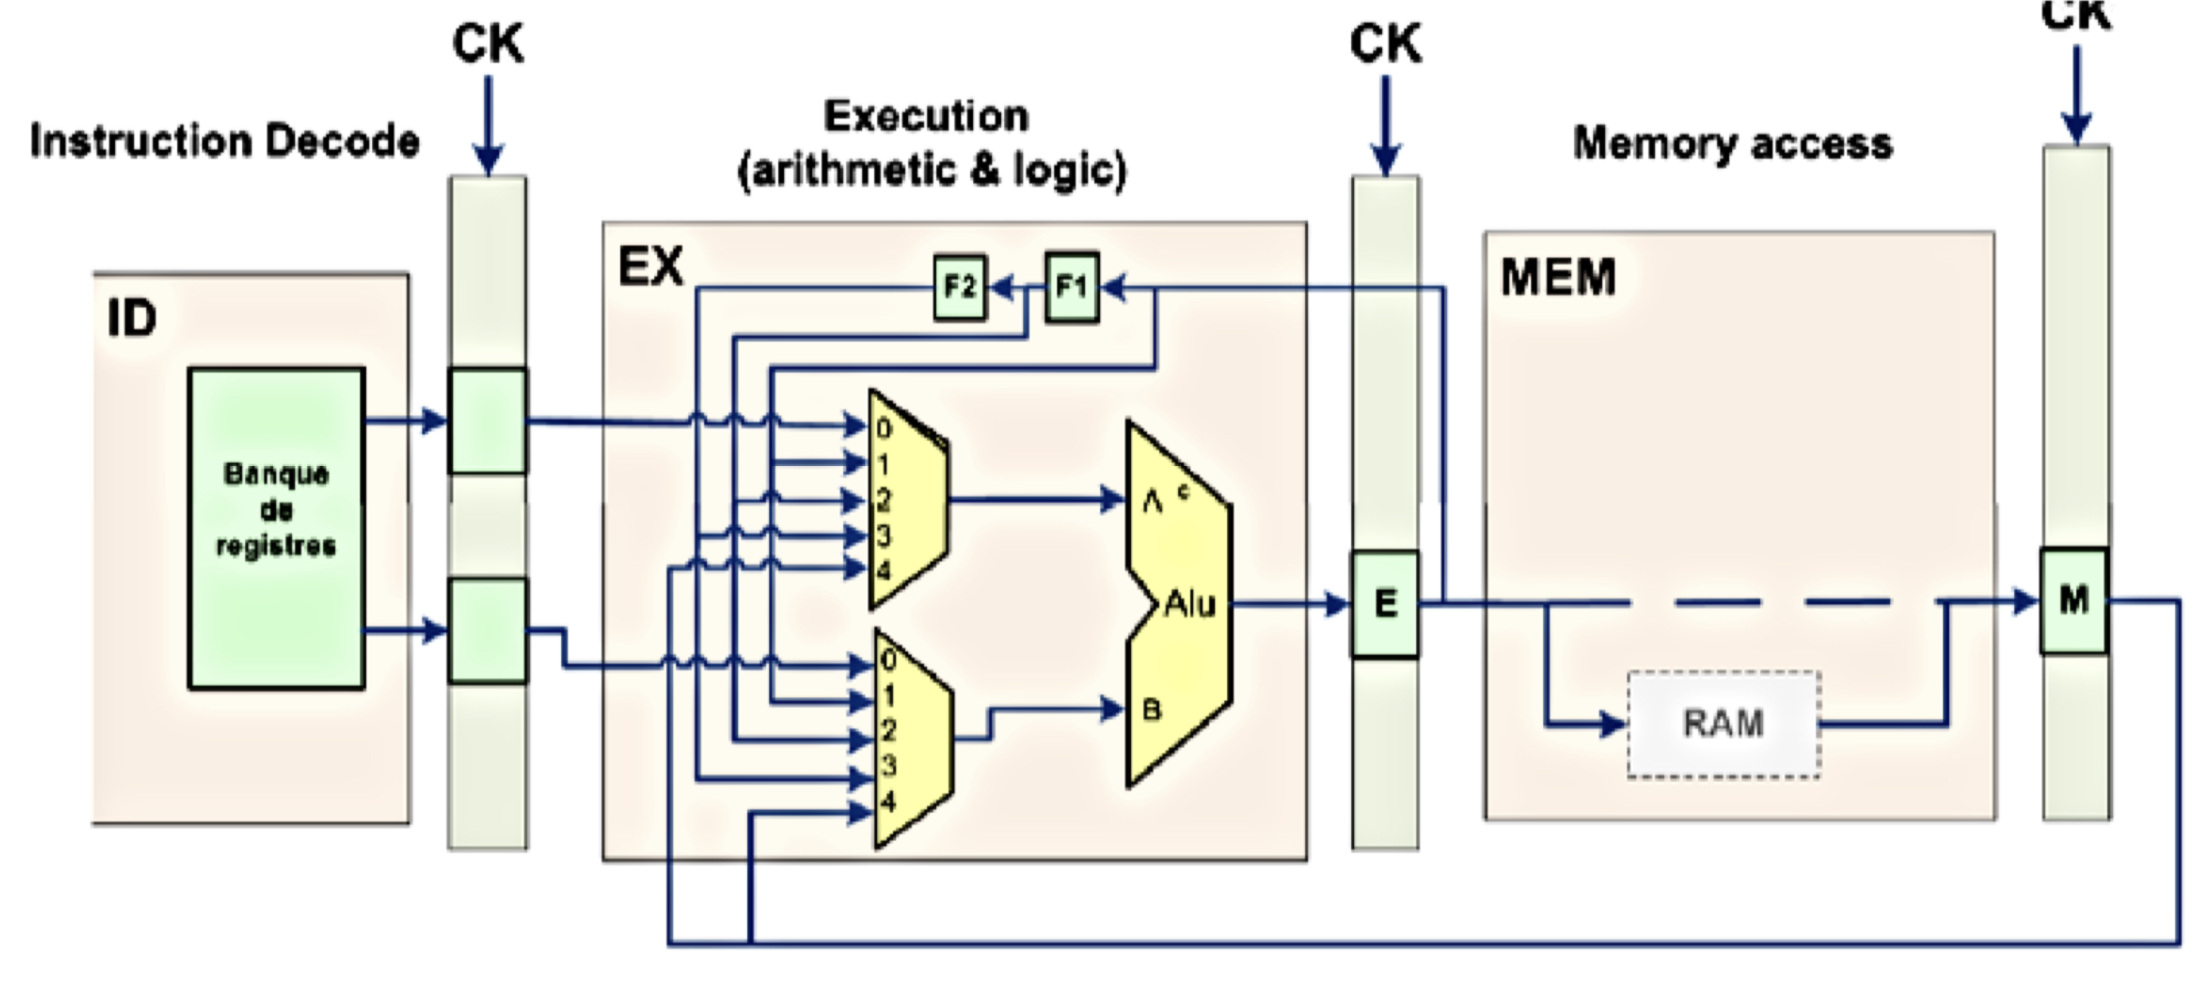
\includegraphics[width=1.1\linewidth]{forwarding_regs.jpeg}
    \end{minipage}
    \begin{minipage}
        \centering
        \rotatebox{-90}{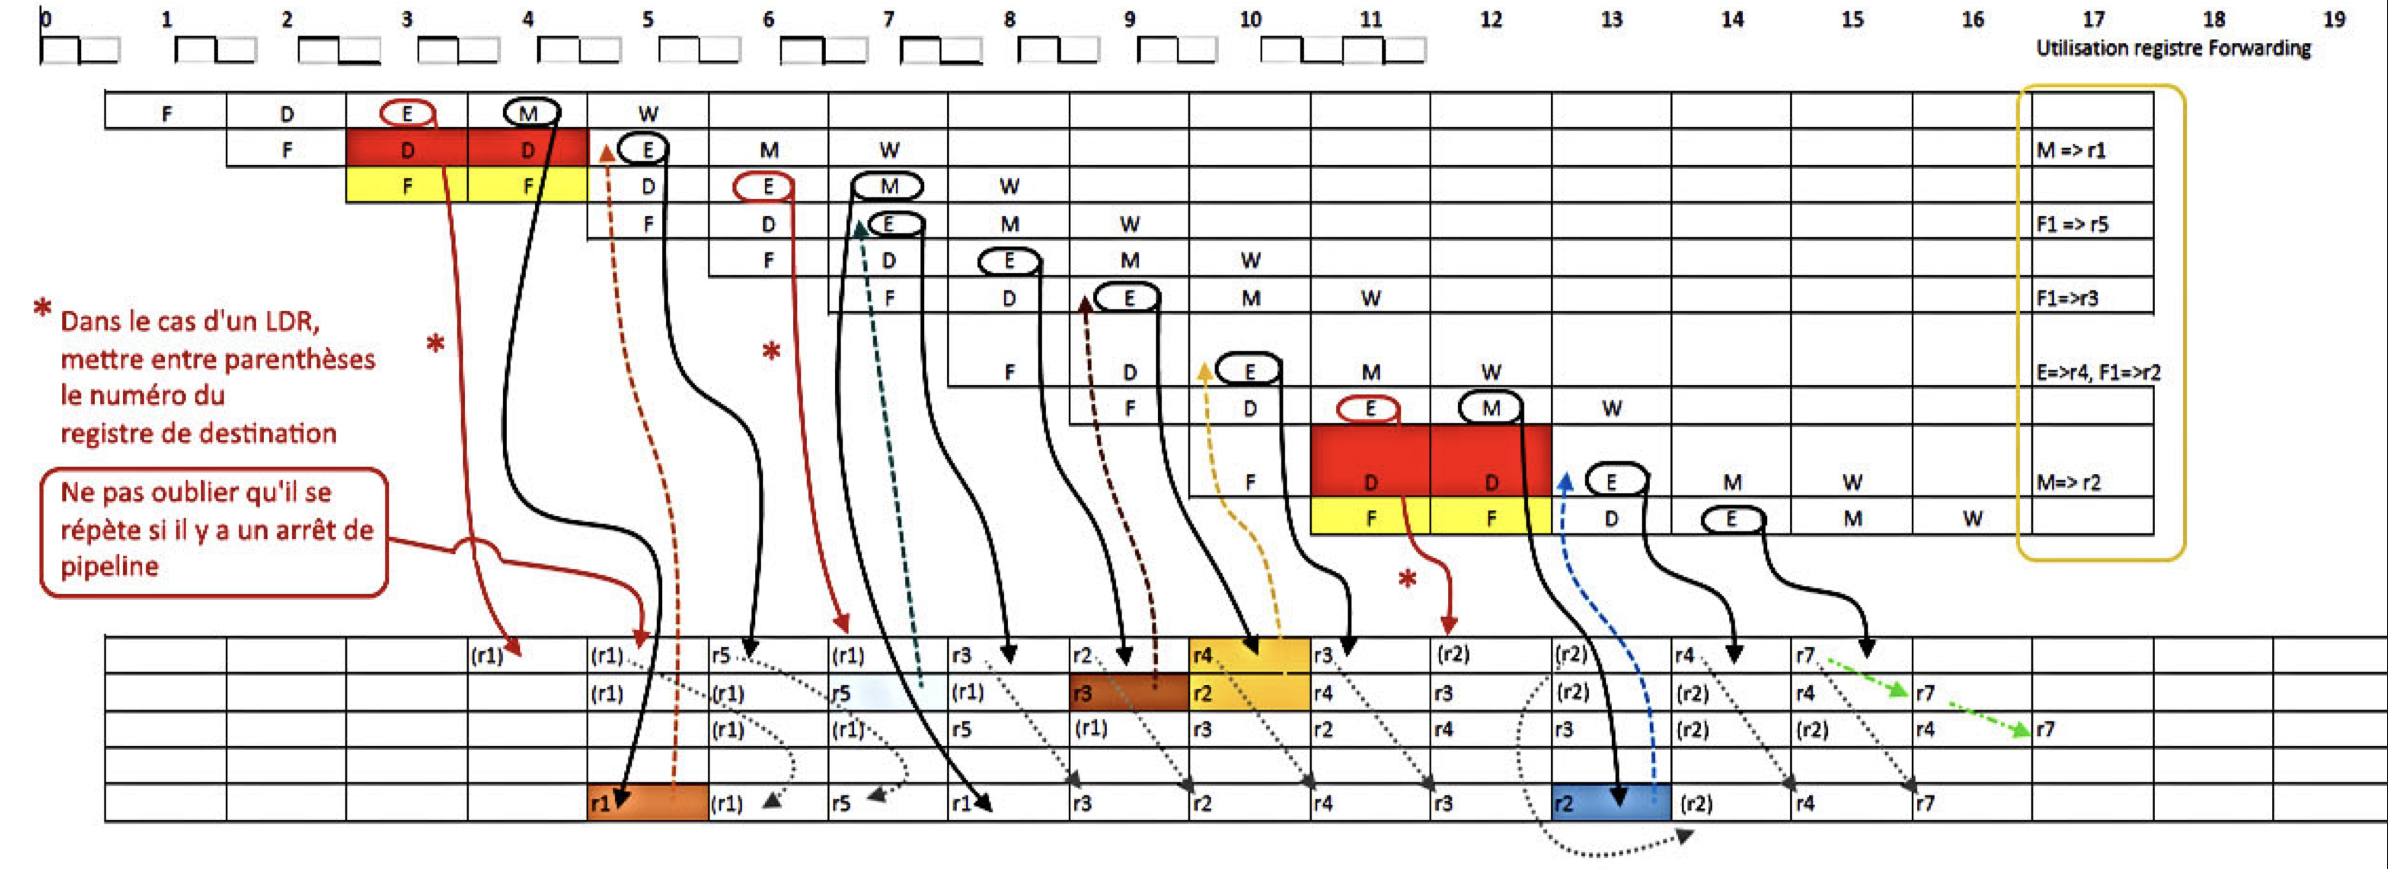
\includegraphics[width=2.4\linewidth]{forwarding.jpeg}}
    \end{minipage}


\end{multicols*}
\end{document}
